\chapter{Risk as Runway: Putting It All on the Line}

This School of Hard Knocks interview, curated for the Entrepreneurship course by LazyingArt LLC, gives us a short but precise study of entrepreneurial risk. The speaker does not begin with a definition. He begins with a newborn on the way, roughly the last \(\$1{,}000\) in the family bank account, a decision to quit and write a first product, the sale of a motorcycle, and then a partner who contributes personal money. We will keep the mathematics close to that sequence: cash buys time, assets can be converted into runway, and risk becomes visible as the gap between a commitment and the resources available to carry it.

\section{The Question: Risk Before Theory}

The opening question asks for the biggest risk the speaker ever took and how important risk has been to him. That order matters. We are not handed a theory and then asked to apply it. We are asked to listen for risk inside a story.

The speaker's first response is simply that it is a good story. That cue should slow us down. The lesson is not a slogan about being bold. It is a small balance-sheet narrative in which family obligations, product-building time, and scarce capital are introduced one by one.

For these notes, we will use \emph{risk} in a deliberately narrow sense. A person has made a commitment, the outcome is uncertain, and the available resources may not be enough to reach the next viable state. In this interview that next viable state is not yet an exit, a valuation, or even a named revenue target. It is enough time to keep building the first product until the venture can find another support point.

\section{The Constraint: A Newborn and the Last Cash}

The first concrete quantity is the remaining cash balance. The speaker says he had a newborn on the way and had gotten down to probably the last \(\$1{,}000\) in his bank account or his wife's bank account. The word ``probably'' matters. We should treat the number as approximate, not audited.

\begin{equation}
C_0 \approx \$1{,}000 .
\end{equation}

Here \(C_0\) denotes the cash available at the point where the story becomes acute. It is not a full statement of net worth. It is the number the speaker gives to make the risk concrete.

\begin{definition}
Runway is the amount of time available before cash runs out, under a given burn rate. If \(C\) is available cash and \(B\) is monthly burn, then the simplest reconstructed runway model is
\begin{equation}
R(C) \approx \frac{C}{B}.
\end{equation}
\end{definition}

The transcript does not give \(B\), so we do not compute a numerical runway. The formula is useful because it names the pressure. With a newborn coming and only about \(\$1{,}000\) left, the problem is no longer just a small cash balance. It is the conversion of dollars into time.

\section{The Decision Point}

The next move is the risky one. The speaker decides to quit and start writing his first product. In the order of the story, this comes after the cash constraint and before the motorcycle sale. That is exactly where it belongs: the decision creates the exposure, and the later actions show how he tries to survive it.

In a product venture, cash is not only a reserve. It is the material that buys uninterrupted work. A month of survival can become a month of writing, testing, selling, or finding help. That does not make the choice safe. It only tells us why the speaker narrates it as a business risk rather than as mere personal hardship.

\subsection{Question \& Answer}

\paragraph{Question.}
Was quitting with a newborn on the way and roughly the last \(\$1{,}000\) in the family bank account calculated risk or recklessness?

\paragraph{Answer.}
The transcript does not give enough information to settle that as a general judgment. What it does show is a sequence of runway extensions. The speaker does not describe a large reserve or a guaranteed investor. He describes a first product, one asset that can be sold, and later a partner who contributes personal money. The risk was extreme, but in the story it is not empty bravado. It is a commitment that has to be carried month by month.

\section{Converting an Asset into Time}

After the decision to quit and build, the speaker sells the one asset he had at the time, a motorcycle. That sale gets them through another month or two. This is the central mathematical move of the interview: an asset is converted into operating time.

Let \(A_{\mathrm{moto}}\) denote the proceeds from selling the motorcycle. The cash update is

\begin{equation}
C_1 = C_0 + A_{\mathrm{moto}} .
\end{equation}

If the monthly burn rate is \(B\), then the added runway from the motorcycle sale is reconstructed as

\begin{equation}
\Delta R_{\mathrm{moto}} \approx \frac{A_{\mathrm{moto}}}{B}.
\end{equation}

The speaker supplies the duration, not the sale price. In cautious notation,

\begin{equation}
\Delta R_{\mathrm{moto}} \approx 1\text{ to }2 \text{ months}.
\end{equation}

This should not be inverted into a motorcycle valuation. We do not know \(A_{\mathrm{moto}}\), and we do not know \(B\). The useful point is structural: a non-cash asset becomes a temporary extension of the time available to build.

\paragraph{A worked runway update.}
The supported calculation is schematic, but it is still a calculation. We begin with the cash constraint, add the asset sale, and express the difference as added runway:

\begin{align}
C_0 &\approx \$1{,}000, \\
C_1 &= C_0 + A_{\mathrm{moto}}, \\
R_0 &\approx \frac{C_0}{B}, \\
R_1 &\approx \frac{C_1}{B}
     = \frac{C_0 + A_{\mathrm{moto}}}{B}, \\
R_1 - R_0 &\approx \frac{A_{\mathrm{moto}}}{B}
          \approx 1\text{ to }2 \text{ months}.
\end{align}

This is as far as the evidence lets us go. The calculation is not meant to make the risk neat. It preserves the speaker's practical logic: the motorcycle sale bought time.

\section{Partner Capital and Shared Exposure}

The next transition is from solitary exposure to shared exposure. The transcript is slightly garbled at this point, but the reliable content is that a future business partner came on board and put in some of his personal money. The story now has a second capital event.

Let \(K_{\mathrm{partner}}\) denote the partner's personal contribution. The next cash state is

\begin{equation}
C_2 = C_1 + K_{\mathrm{partner}}
    = C_0 + A_{\mathrm{moto}} + K_{\mathrm{partner}} .
\end{equation}

The corresponding reconstructed runway is

\begin{equation}
R_2 \approx \frac{C_0 + A_{\mathrm{moto}} + K_{\mathrm{partner}}}{B}.
\end{equation}

Again, the numbers are not available. We do not know the contribution, the burn rate, the equity arrangement, the product timeline, or the eventual company economics. But the rhythm of the story is clear. First there is the household cash constraint. Then the founder converts a personal asset into another month or two. Then a partner contributes personal money. The risk remains real, but it is no longer carried by one person in exactly the same way.

\section{The Sequence as a Runway Diagram}

The following figure is a transcript-derived reconstruction. It is not a copied board diagram. Its job is to keep the business mechanism visible in the same order in which the speaker gives it.

\begin{figure}
\centering
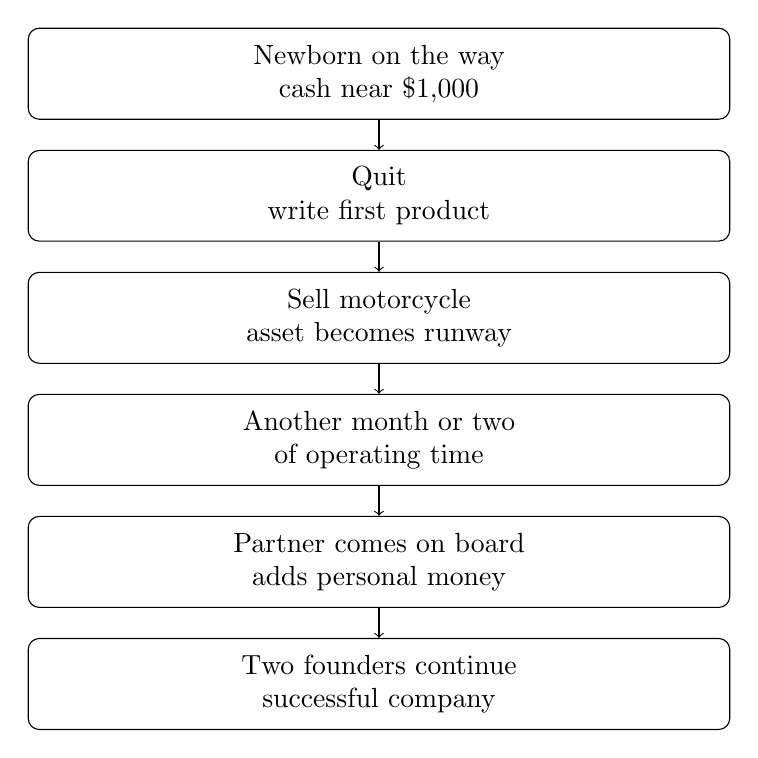
\begin{tikzpicture}[x=1cm,y=1cm]
\node[draw, rounded corners, align=center, text width=0.70\linewidth, inner sep=6pt] (a) at (0,0)
{Newborn on the way\\cash near \(\$1{,}000\)};

\node[draw, rounded corners, align=center, text width=0.70\linewidth, inner sep=6pt] (b) at (0,-1.55)
{Quit\\write first product};

\node[draw, rounded corners, align=center, text width=0.70\linewidth, inner sep=6pt] (c) at (0,-3.10)
{Sell motorcycle\\asset becomes runway};

\node[draw, rounded corners, align=center, text width=0.70\linewidth, inner sep=6pt] (d) at (0,-4.65)
{Another month or two\\of operating time};

\node[draw, rounded corners, align=center, text width=0.70\linewidth, inner sep=6pt] (e) at (0,-6.20)
{Partner comes on board\\adds personal money};

\node[draw, rounded corners, align=center, text width=0.70\linewidth, inner sep=6pt] (f) at (0,-7.75)
{Two founders continue\\successful company};

\draw[->] (a) -- (b);
\draw[->] (b) -- (c);
\draw[->] (c) -- (d);
\draw[->] (d) -- (e);
\draw[->] (e) -- (f);
\end{tikzpicture}
\caption{A transcript-derived runway sequence: cash constraint, product work, asset liquidation, partner capital, and eventual company success.}
\end{figure}

The diagram also explains why the closing sentence has force. The phrase ``all on the line'' is not just emotional emphasis. It summarizes a chain in which nearly all available resources were committed before the outcome was secure.

\section{Putting It All on the Line}

The final claim is that saying he put it all on the line is not an understatement. We should not soften that line into a general moral about risk-taking. Nor should we let the later success erase the uncertainty at the time of the decision. The point is sharper if we keep both facts together: the company became successful, and the early exposure was severe.

The capital sequence can be summarized compactly:

\begin{align}
C_0 &\approx \$1{,}000, \\
C_1 &= C_0 + A_{\mathrm{moto}}, \\
C_2 &= C_1 + K_{\mathrm{partner}}.
\end{align}

Each update corresponds to a spoken beat. The first line is the family cash constraint. The second is the motorcycle sale. The third is the partner's personal contribution. If we preserve that order, we preserve the commercial reasoning of the story.

A more general shortfall expression would require assumptions the interview does not supply. If a product effort requires \(T\) months, then a reconstructed cash shortfall at that horizon would have the form

\begin{equation}
S(T) = BT - C_2 .
\end{equation}

But this should remain a conceptual aid, not a reported fact. The interview does not state \(T\), \(B\), or \(C_2\) numerically. What it states is the lived version: there was almost no cushion, an asset was sold for another month or two, and a partner's personal money helped carry the venture forward.

\section{Summary}

This chapter's mathematical payload is small but sharp. Risk is treated as runway under pressure. The speaker begins with a newborn on the way and roughly the last \(\$1{,}000\), chooses to quit and write a first product, sells the one asset he names, gains another month or two, and then survives long enough for a partner to contribute personal money.

We should not add a theory that the interview does not provide. There is no probability model, valuation, equity calculation, or detailed company chronology here. What the transcript gives us is a disciplined sequence: scarce cash, product commitment, asset liquidation, partner capital, and the retrospective recognition that the founder really did put everything on the line.